\documentclass[11pt,a4paper]{article}
\usepackage[margin=25mm]{geometry}
\usepackage{amsmath,amssymb,bm,graphicx,booktabs,microtype,upgreek}
\usepackage[colorlinks=true,allcolors=blue]{hyperref}
\usepackage{caption}
\captionsetup{font=small,labelfont=bf}
\renewcommand{\arraystretch}{1.15}
\title{Altitude response of a free-falling permeable plate\\to a fluctuation of the gravitational acceleration}
\author{Ignazio Maria Viola\\ School of Engineering, University of Edinburgh}
\date{14 September 2026}
\begin{document}\maketitle

\begin{abstract}
\noindent We quantify how a transient fluctuation of the gravitational
acceleration displaces a two-dimensional free-falling permeable plate, using
direct numerical simulations at a Galilei number $Ga=150$. A plate free to
rotate either gains or loses altitude, according to the order in which the
vertical component $g_y$ is raised and lowered. When the angular position is
constrained, every case tested gains altitude, irrespective of that order. A
fluctuation of the horizontal component $g_x$ always produces a gain, between
one and two orders of magnitude larger than for $g_y$. The results are limited
to Darcy numbers $Da=10^{-5}$ and $10^{-4}$ for the constrained plate, and the
horizontal cases have not recovered their descent speed within the simulated
window, so the reported gains are lower bounds.
\end{abstract}

\section{Introduction}

A body falling freely in a fluid does not respond to a transient perturbation
of its weight by returning to its original trajectory. The perturbation leaves
a residual displacement even when it carries no net impulse, and the sign and
magnitude of that displacement are not obvious \emph{a priori}. This report
quantifies the residual altitude change of a permeable plate for fluctuations
of the vertical and of the horizontal component of the gravitational
acceleration.

All symbols are nondimensional unless carrying a hat, in which case they are
dimensional. Lengths are scaled on the plate length $c$, velocities on the
gravitational velocity $u_g \equiv (\hat m \hat g/\hat\rho \hat c^2)^{1/2}$,
and the fluid density is unity.

\section{Methodology}

\subsection{Governing parameters}

The flow is governed by the Galilei number $Ga \equiv u_g c/\nu$, where $\nu$
is the kinematic viscosity; the Darcy number $Da \equiv K/c^2$, where $K$ is
the permeability; the nondimensional mass $m$; the chord-to-thickness ratio
$\chi \equiv c/f$, where $f$ is the thickness; the nondimensional moment of
inertia $I_O$ about the plate centre; and the offset $e$ of the centre of
gravity from that centre along the body normal. The solid volume is neglected,
so buoyancy is null and the nondimensional gravitational acceleration is
$g=1/m$.

We take $Ga=150$, $\chi=10$, $m=0.80$, $e=1.16$ and $I_O=1.15$ throughout, and
vary $Da$ between $10^{-5}$ and $10^{-3}$.

\subsection{Gravity fluctuation}

The fluctuation is applied over a single period $T_G=2$ convective times
beginning at $t_0$, as a transient change of the gravitational acceleration,
\begin{equation}
  \bm{g}_\mathrm{eff}(t) = \bm{g} \pm A\,g\sin\!\left[\frac{2\uppi(t-t_0)}{T_G}\right]\bm{e},
  \label{eq:gust}
\end{equation}
where $A$ is the semi-amplitude as a fraction of $g$; $\bm{e}$ is the
direction of the fluctuation, $\bm{e}_y$ for a fluctuation of the vertical
component and $\bm{e}_x$ for the horizontal; and the sign selects the order in
which the two excursions occur. The net impulse of equation~\eqref{eq:gust} is
null, so the fluctuation changes neither the mean nor the final gravitational
force. For $A\ge 1.5$ applied vertically the effective gravity reverses during
part of the period.

\subsection{Numerical method}

The incompressible Navier--Stokes equations are solved with the boundary data
immersion method (BDIM) on a uniform Cartesian grid, in a frame translating
with the plate. Permeability enters as a Brinkman resistance blended into the
BDIM mobility, which recovers the impermeable body exactly as $Da\to 0$. Three
degrees of freedom are integrated with the added-mass tensor treated
implicitly. The plate length is 64 cells, giving 6.4 cells across the
thickness, in a domain of $16c \times 16c$.

Each configuration is first advanced from rest to its terminal state, then
branched: one continuation at constant gravity as a reference, and one per
fluctuation. All branches of a configuration start from an identical saved
state, so the difference between them is due to the fluctuation alone. The
altitude change is
\begin{equation}
  \Delta Y(t) \equiv Y(t) - Y_\mathrm{ref}(t),
  \label{eq:dy}
\end{equation}
where $Y_\mathrm{ref}$ is the altitude of the reference plate, so that
$\Delta Y > 0$ denotes a gain.

\section{Results}

\subsection{Plates free to rotate}

A plate free to rotate either gains or loses altitude, and which of the two
occurs is set by the order of the fluctuation (figure~\ref{fig:free}).
Reducing $g_y$ first produces a gain, and raising it first produces a loss, at
every amplitude tested. The response is close to antisymmetric: the residual
sum $\Delta Y_\downarrow + \Delta Y_\uparrow$ is $-0.0025$, $+0.0234$ and
$-0.0231$ for $A=0.5$, $1.5$ and $2.5$, against individual responses of order
$0.1$.

The outcome is therefore deterministic rather than uncertain. The sign of the
residual follows the sign of the first excursion, and reversing the order
reverses the displacement.

\begin{figure}[htbp]\centering
  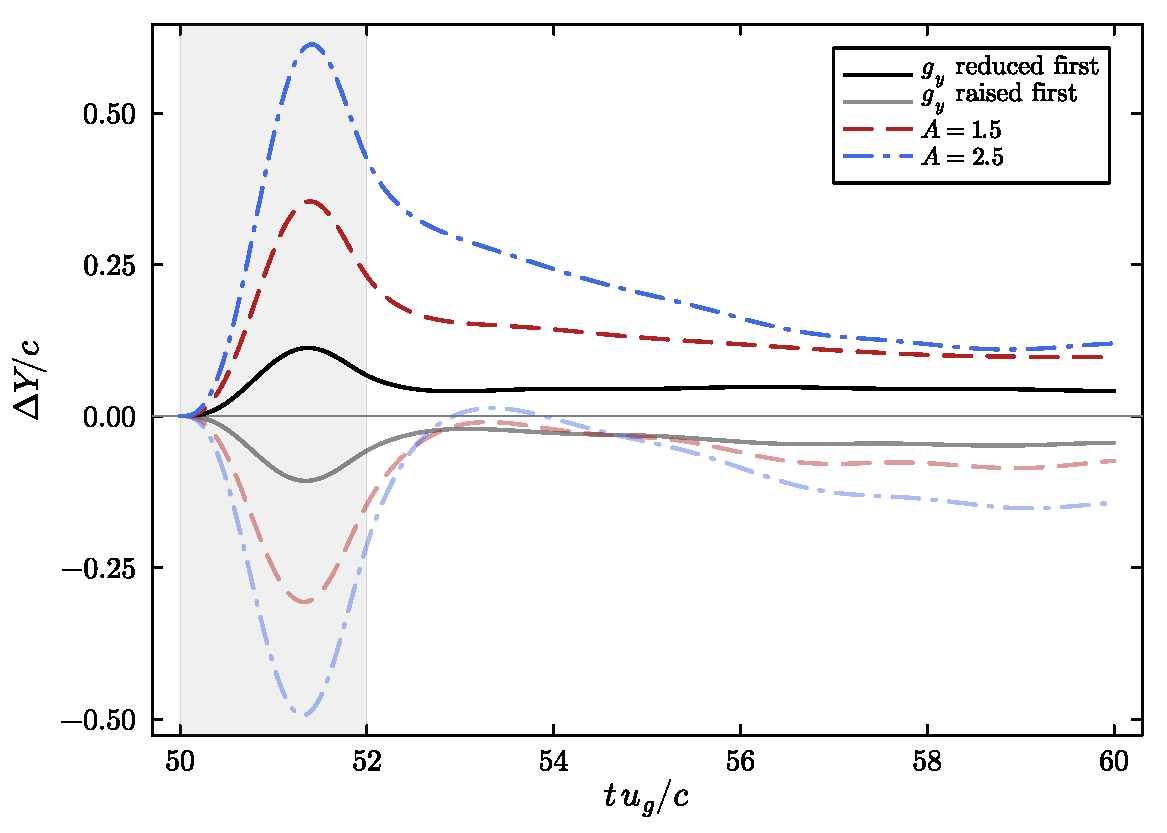
\includegraphics[width=0.62\textwidth]{fig1.pdf}
  \caption{Altitude change versus time for a plate free to rotate, for values
  of the semi-amplitude $A$ from 0.5 to 2.5 and both orders of the fluctuation,
  for $Da=10^{-4}$. The shaded band is the fluctuation period.}
  \label{fig:free}
\end{figure}

\subsection{Plates with a fixed angular position}

When the angular position is constrained, every plate tested gains altitude
(figure~\ref{fig:fixed}). This holds at both Darcy numbers and at all three
amplitudes, for both orders of the fluctuation: all twelve residuals are
positive, between $+0.004$ and $+0.211$.

Constraining the rotation therefore removes the part of the response whose sign
follows the order, and leaves a rectified part that displaces the plate upwards
whichever way the fluctuation runs. Decomposing the residual into a component
that changes sign with the order and one that does not, the former falls by a
factor between three and eight when the rotation is constrained, while the
latter rises from at most $0.012$ to $0.167$.

\begin{figure}[htbp]\centering
  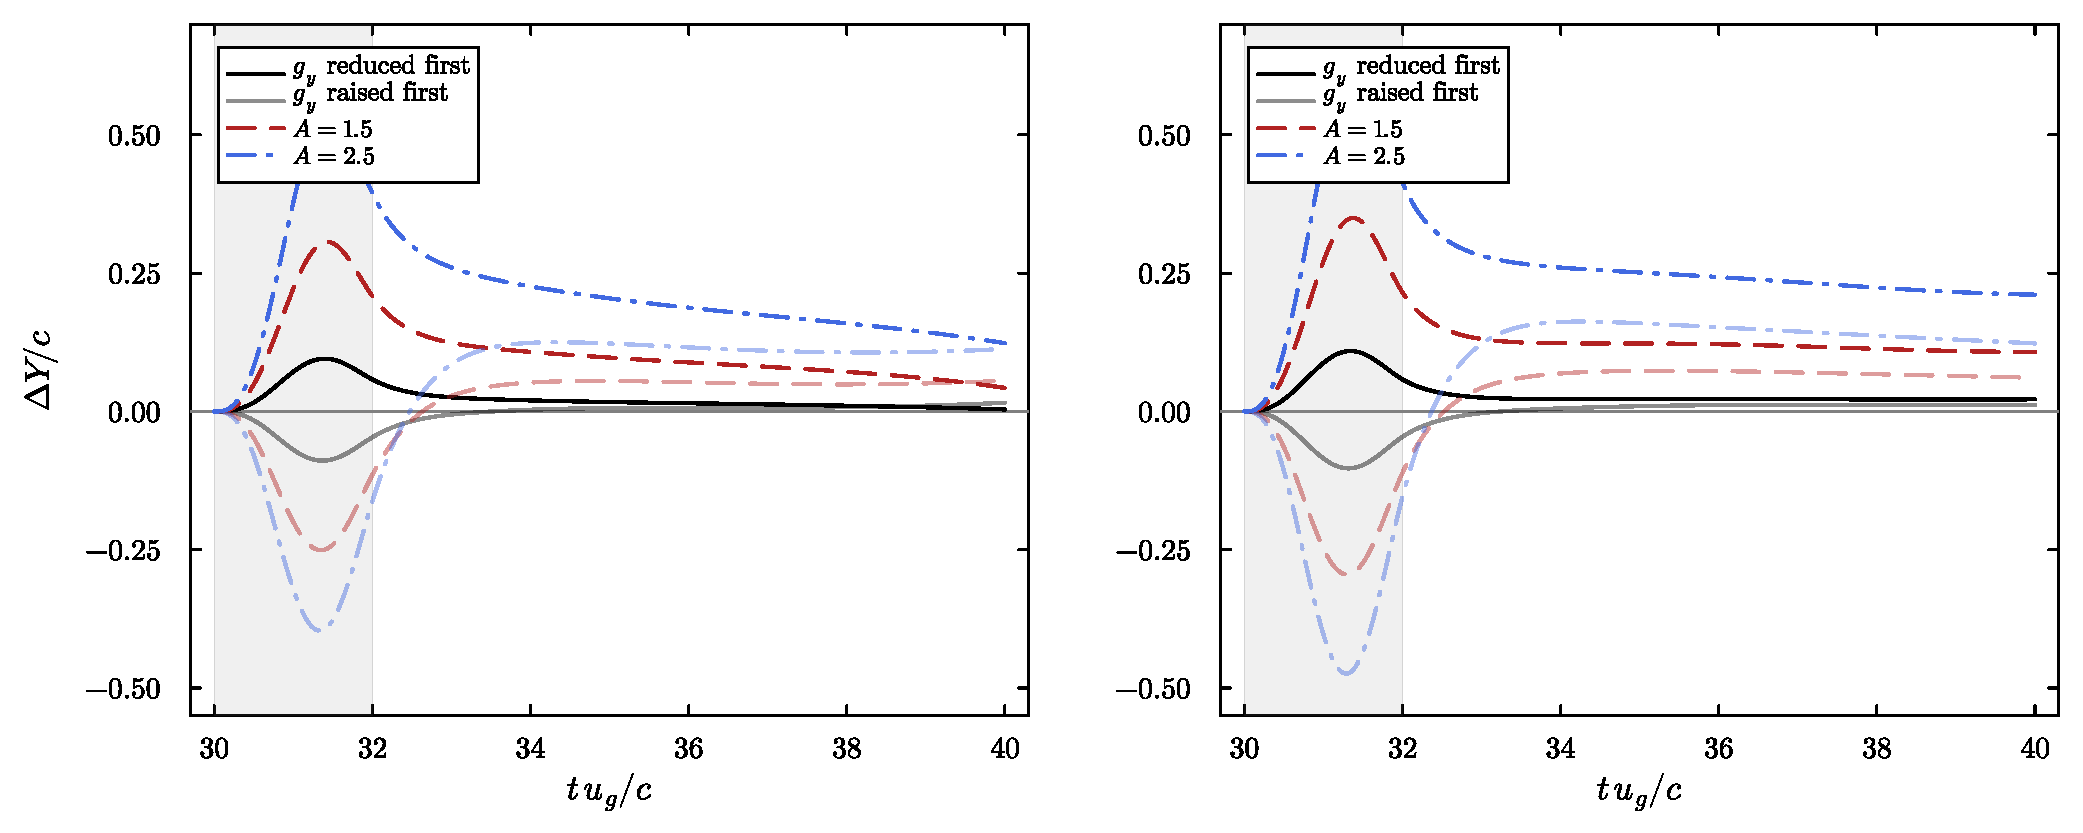
\includegraphics[width=\textwidth]{fig2.pdf}
  \caption{Altitude change versus time for a plate with a fixed angular
  position, for values of the semi-amplitude $A$ from 0.5 to 2.5 and both
  orders of the fluctuation: (a) $Da=10^{-5}$, (b) $Da=10^{-4}$. The shaded
  band is the fluctuation period.}
  \label{fig:fixed}
\end{figure}

\subsection{Fluctuation of the horizontal component}

A fluctuation of $g_x$ always produces an altitude gain, at every Darcy number
and amplitude tested, and for both signs (figure~\ref{fig:horiz}). The vertical
component of gravity is constant throughout these simulations, so the gain is
produced entirely by the lateral forcing.

The gain is between one and two orders of magnitude larger than that produced
by a fluctuation of $g_y$ of the same amplitude (figure~\ref{fig:compare} and
table~\ref{tab:ratio}). It is also rectified to a closer tolerance: at
$Da=10^{-4}$ and $A=2.5$ the two signs give $+2.119$ and $+2.106$, a difference
of 0.6\%.

\begin{figure}[htbp]\centering
  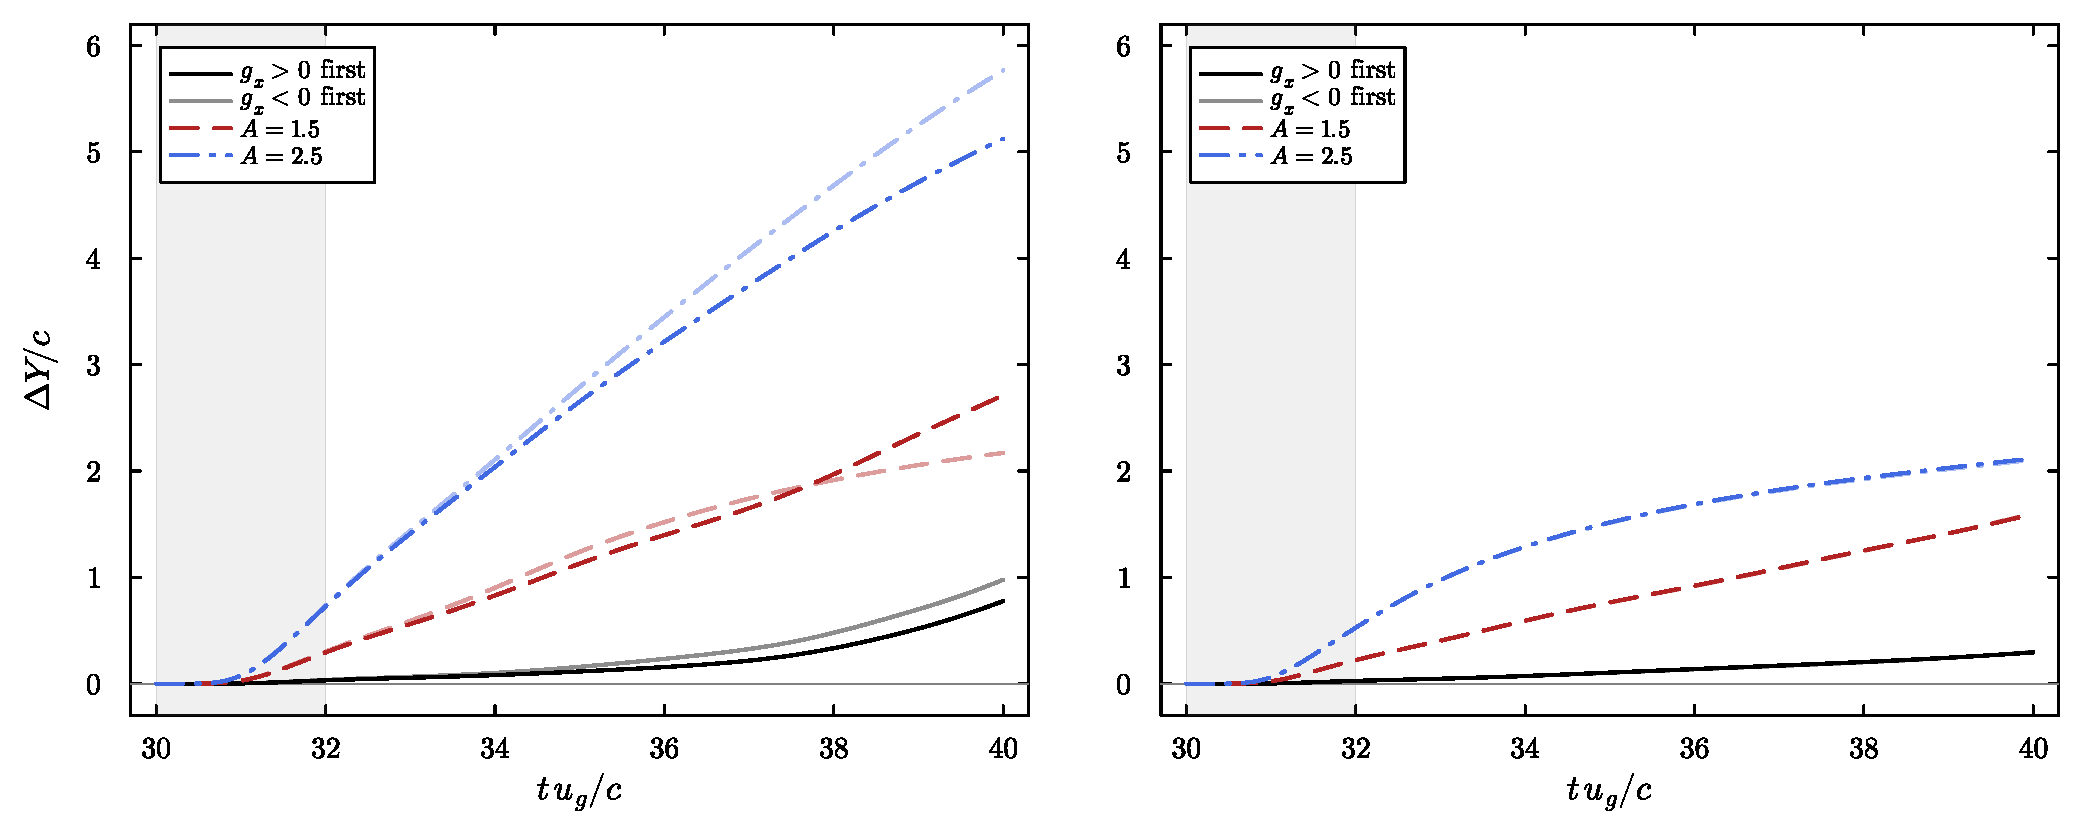
\includegraphics[width=\textwidth]{fig3.pdf}
  \caption{Altitude change versus time for a fluctuation of the horizontal
  component of the gravitational acceleration, for a plate with a fixed angular
  position, for values of the semi-amplitude $A$ from 0.5 to 2.5 and both signs:
  (a) $Da=10^{-5}$, (b) $Da=10^{-4}$. The shaded band is the fluctuation period.
  Note the ordinate range, ten times that of figure~\ref{fig:fixed}.}
  \label{fig:horiz}
\end{figure}

\begin{table}[htbp]\centering
  \caption{Altitude gain ten convective times after the onset of the
  fluctuation, averaged over the two orders, and the ratio between the
  horizontal and the vertical fluctuation, for a plate with a fixed angular
  position.}
  \label{tab:ratio}
  \begin{tabular}{ccccc}
    \toprule
    $Da$ & $A$ & $\Delta Y/c$, $g_x$ & $\Delta Y/c$, $g_y$ & ratio \\
    \midrule
    $10^{-5}$ & 0.5 & 0.878 & 0.010 & 90 \\
    $10^{-5}$ & 1.5 & 2.441 & 0.049 & 50 \\
    $10^{-5}$ & 2.5 & 5.445 & 0.118 & 46 \\
    $10^{-4}$ & 0.5 & 0.297 & 0.017 & 18 \\
    $10^{-4}$ & 1.5 & 1.601 & 0.084 & 19 \\
    $10^{-4}$ & 2.5 & 2.112 & 0.167 & 13 \\
    \bottomrule
  \end{tabular}
\end{table}

\begin{figure}[htbp]\centering
  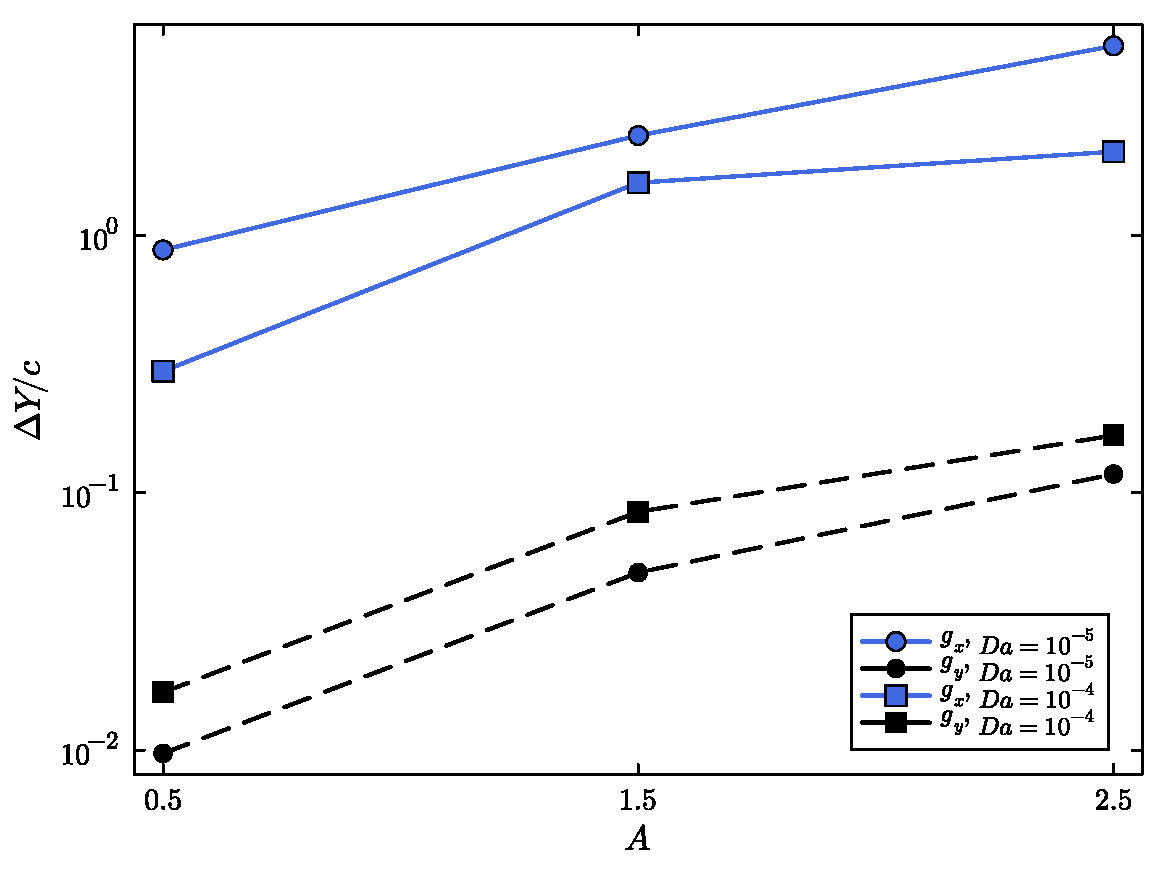
\includegraphics[width=0.62\textwidth]{fig4.pdf}
  \caption{Altitude gain ten convective times after the onset of the
  fluctuation versus semi-amplitude, for fluctuations of the horizontal and of
  the vertical component of the gravitational acceleration, for $Da=10^{-5}$
  and $10^{-4}$, for a plate with a fixed angular position.}
  \label{fig:compare}
\end{figure}

\section{Caveats}

Four limitations bound the results.

\textbf{Limited range of $Da$.} The constrained-rotation results of
sections~3.2 and 3.3 cover only $Da=10^{-5}$ and $10^{-4}$, a single decade.
The statement that every constrained plate gains altitude is therefore
established over that decade and not over the wider range $10^{-5}$ to
$10^{-3}$ explored for the plate free to rotate.

\textbf{Time histories not converged for a horizontal fluctuation.} For a
fluctuation of $g_y$ the altitude change settles within the simulated window,
and the descent speed returns to its reference value to within 0.5\%. For a
fluctuation of $g_x$ it does not: ten convective times after the onset the
plate is still descending between 7\% ($Da=10^{-4}$) and 38\% ($Da=10^{-5}$)
more slowly than the reference, and $\Delta Y$ is still growing. The gains of
section~3.3 are therefore lower bounds, and the ratios of
table~\ref{tab:ratio} depend on the instant at which they are evaluated.

\textbf{Mechanisms are not established.} Only the trajectories and the
integrated loads were recorded. No force decomposition, quasi-steady baseline
or flow-field data was collected, so no mechanism is demonstrated and none is
claimed here.

\textbf{Numerical resolution.} The Brinkman screening length $c\sqrt{Da}$ is
0.64 and 0.20 cells at $Da=10^{-4}$ and $10^{-5}$, so the internal layer is
not resolved; for a thin plate the governing quantity is the pressure drop
across it, which does not require it. No grid-convergence study was made. The
comparisons are between simulations at identical resolution and are therefore
robust to a common discretisation error, but absolute values are not
established. In the most displaced case the plate moves 3.4 chords laterally
in a domain 16 chords wide with periodic lateral boundaries, and interaction
with its own periodic image is untested.

\section{Conclusions}

Three results follow from 47 simulations at $Ga=150$.

A plate free to rotate either gains or loses altitude in response to a
fluctuation of the vertical component of the gravitational acceleration,
according to the order in which that component is raised and lowered.

A plate whose angular position is fixed gains altitude in every case tested,
at both Darcy numbers and all three amplitudes, and for both orders.

A fluctuation of the horizontal component always produces a gain, between one
and two orders of magnitude larger than for the vertical component at the same
amplitude, evaluated ten convective times after the onset.

\vspace{2mm}\noindent
Code and data: \url{https://github.com/ignaziomviola/FallingPlate2D.jl}.

\end{document}
